\subsubsection{Vigas auxiliares piso tipo}
\begin{itemize}
        \item \textbf{Viga auxiliar 10}\\
            \begin{figure}[H]
                \centering
                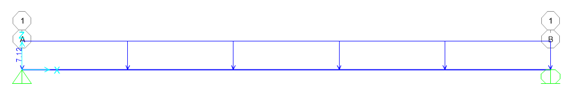
\includegraphics[width=0.9\linewidth]{images/viguetas/V-10.png}
                \caption{Diagrama de carga (1.2D+1.6L) para la viga auxiliar V-10 de entrepiso}
                \label{fig:W V-10 EP}
            \end{figure}
            
            \begin{figure}[H]
                \centering
                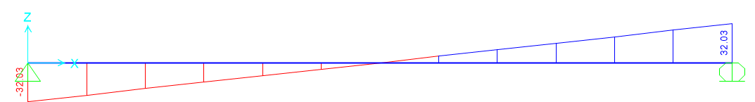
\includegraphics[width=0.9\linewidth]{images/viguetas/CORT-10.png}
                \caption{Diagrama de cortante (1.2D+1.6L) para la viga auxiliar V-10 de entrepiso}
                \label{fig:Cort V-10 EP}
            \end{figure}
            
            \begin{figure}[H]
                \centering
                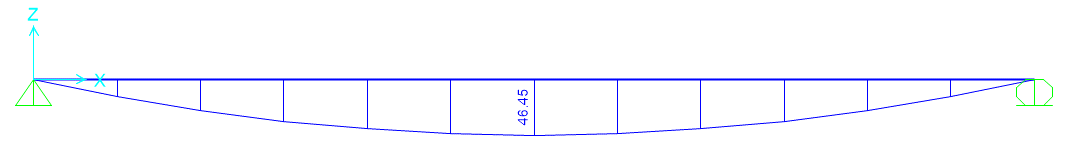
\includegraphics[width=0.9\linewidth]{images/viguetas/MOM-10.png}
                \caption{Diagrama de momento (1.2D+1.6L) para la viga auxiliar V-10 de entrepiso}
                \label{fig:MOm V-10 EP}
            \end{figure}
            
            \item \textbf{Viga auxiliar 11}\\
            \begin{figure}[H]
                \centering
                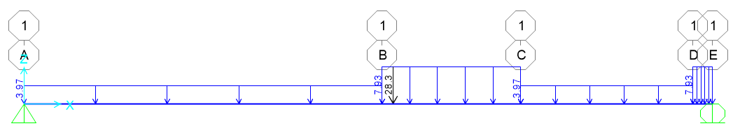
\includegraphics[width=0.9\linewidth]{images/viguetas/V-11.png}
                \caption{Diagrama de carga (1.2D+1.6L) para la viga auxiliar V-11 de entrepiso}
                \label{fig:W V-11 EP}
            \end{figure}
            
            \begin{figure}[H]
                \centering
                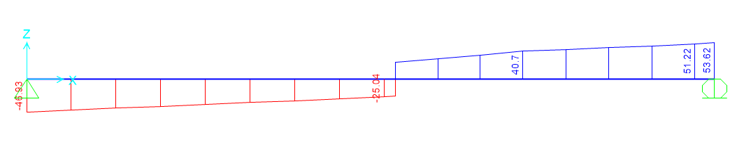
\includegraphics[width=0.9\linewidth]{images/viguetas/CORT-11.png}
                \caption{Diagrama de cortante (1.2D+1.6L) para la viga auxiliar V-11 de entrepiso}
                \label{fig:Cort V-11 EP}
            \end{figure}
            
            \begin{figure}[H]
                \centering
                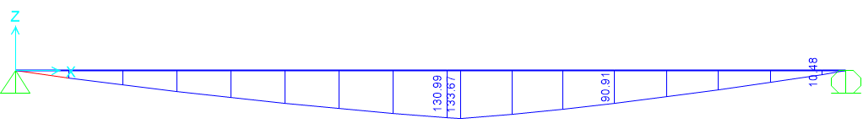
\includegraphics[width=0.9\linewidth]{images/viguetas/MOM-11.png}
                \caption{Diagrama de momento (1.2D+1.6L) para la viga auxiliar V-11 de entrepiso}
                \label{fig:Mom V-11 EP}
            \end{figure}
            
            \item \textbf{Viga auxiliar 12}\\
            \begin{figure}[H]
                \centering
                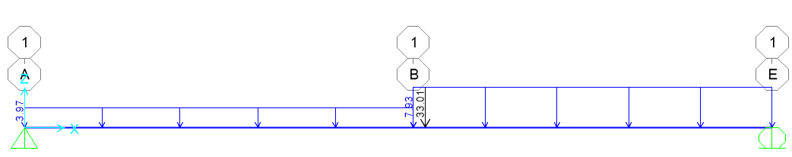
\includegraphics[width=0.9\linewidth]{images/viguetas/V-12.png}
                \caption{Diagrama de carga (1.2D+1.6L) para la viga auxiliar V-12 de entrepiso}
                \label{fig:W V-12 EP}
            \end{figure}
            
            \begin{figure}[H]
                \centering
                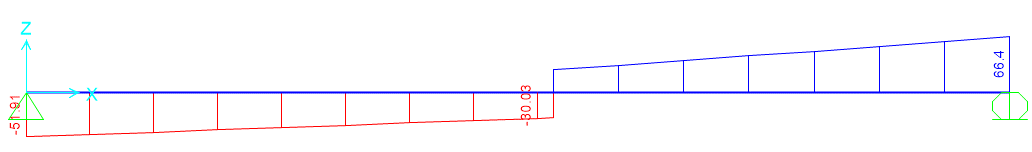
\includegraphics[width=0.9\linewidth]{images/viguetas/CORT-12.png}
                \caption{Diagrama de cortante (1.2D+1.6L) para la viga auxiliar V-12 de entrepiso}
                \label{fig:Cort V-12 EP}
            \end{figure}
            
            \begin{figure}[H]
                \centering
                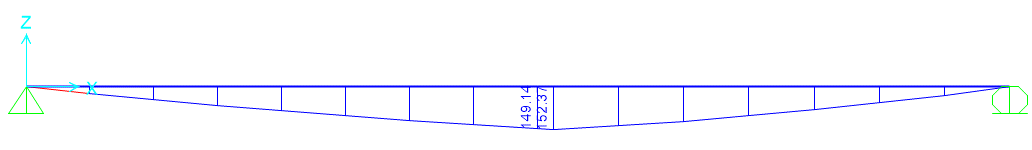
\includegraphics[width=0.9\linewidth]{images/viguetas/MOM-12.png}
                \caption{Diagrama de momento (1.2D+1.6L) para la viga auxiliar V-12 de entrepiso}
                \label{fig:Mom V-12 EP}
            \end{figure}
            
            
            \item \textbf{Viga auxiliar 13}\\
            \begin{figure}[H]
                \centering
                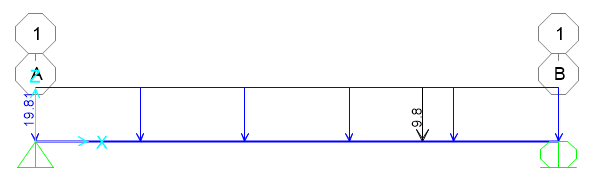
\includegraphics[width=0.9\linewidth]{images/viguetas/V-13.png}
                \caption{Diagrama de carga (1.2D+1.6L) para la viga auxiliar V-13 de entrepiso}
                \label{fig:W V-13 EP}
            \end{figure}
            
            \begin{figure}[H]
                \centering
                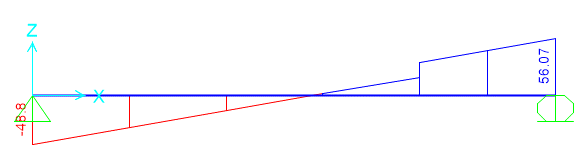
\includegraphics[width=0.9\linewidth]{images/viguetas/CORT-13.png}
                \caption{Diagrama de cortante (1.2D+1.6L) para la viga auxiliar V-13 de entrepiso}
                \label{fig:Cort V-13 EP}
            \end{figure}
            
            \begin{figure}[H]
                \centering
                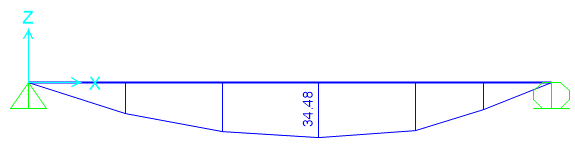
\includegraphics[width=0.9\linewidth]{images/viguetas/MOM-13.png}
                \caption{Diagrama de momento (1.2D+1.6L) para la viga auxiliar V-13 de entrepiso}
                \label{fig:Mom V-13 EP}
            \end{figure}
            
            \item \textbf{Viga auxiliar 14}\\
            \begin{figure}[H]
                \centering
                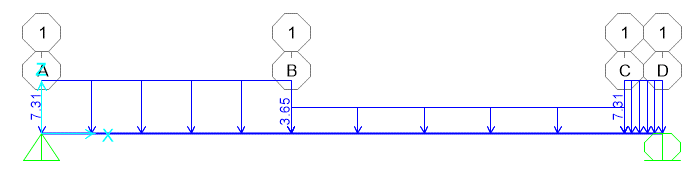
\includegraphics[width=0.9\linewidth]{images/viguetas/V-14.png}
                \caption{Diagrama de carga (1.2D+1.6L) para la viga auxiliar V-14 de entrepiso}
                \label{fig:W V-14 EP}
            \end{figure}
            
            \begin{figure}[H]
                \centering
                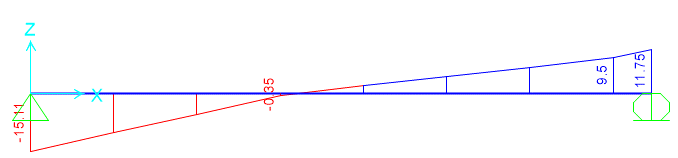
\includegraphics[width=0.9\linewidth]{images/viguetas/CORT-14.png}
                \caption{Diagrama de cortante (1.2D+1.6L) para la viga auxiliar V-14 de entrepiso}
                \label{fig:Cort V-14 EP}
            \end{figure}
            
            \begin{figure}[H]
                \centering
                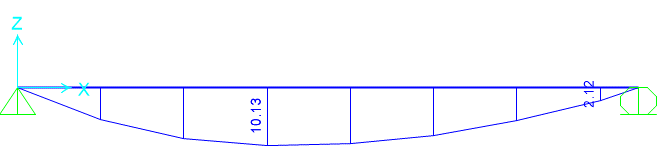
\includegraphics[width=0.9\linewidth]{images/viguetas/MOM-14.png}
                \caption{Diagrama de momento (1.2D+1.6L) para la viga auxiliar V-14 de entrepiso}
                \label{fig:Mom V-14 EP}
            \end{figure}
            
\end{itemize}




\subsubsection{Vigas auxiliares cubierta}
\begin{itemize}
        % \item \textbf{Viga auxiliar 10}\\
        %     \begin{figure}[H]
        %         \centering
        %         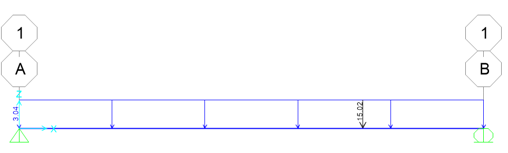
\includegraphics[width=0.9\linewidth]{images/viguetas/V-10C.png}
        %         \caption{Diagrama de carga (1.2D+1.6L) para la viga auxiliar V-10 de cubierta}
        %         \label{fig:W V-10 EP}
        %     \end{figure}
            
        %     \begin{figure}[H]
        %         \centering
        %         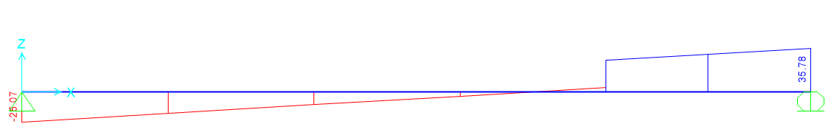
\includegraphics[width=0.9\linewidth]{images/viguetas/CORT-10C.png}
        %         \caption{Diagrama de cortante (1.2D+1.6L) para la viga auxiliar V-10 de cubierta}
        %         \label{fig:Cort V-10 EP}
        %     \end{figure}
            
        %     \begin{figure}[H]
        %         \centering
        %         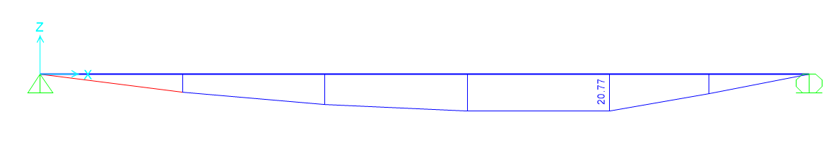
\includegraphics[width=0.9\linewidth]{images/viguetas/MOM-10C.png}
        %         \caption{Diagrama de momento (1.2D+1.6L) para la viga auxiliar V-10 de cubierta}
        %         \label{fig:MOm V-10 EP}
        %     \end{figure}
            
            \item \textbf{Viga auxiliar 11}\\
            \begin{figure}[H]
                \centering
                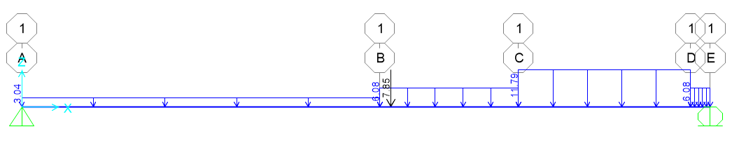
\includegraphics[width=0.9\linewidth]{images/viguetas/V-11C.png}
                \caption{Diagrama de carga (1.2D+1.6L) para la viga auxiliar V-11 de cubierta}
                \label{fig:W V-11 EP}
            \end{figure}
            
            \begin{figure}[H]
                \centering
                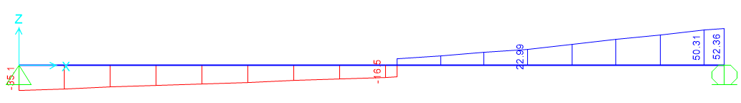
\includegraphics[width=0.9\linewidth]{images/viguetas/CORT-11C.png}
                \caption{Diagrama de cortante (1.2D+1.6L) para la viga auxiliar V-11 de cubierta}
                \label{fig:Cort V-11 EP}
            \end{figure}
            
            \begin{figure}[H]
                \centering
                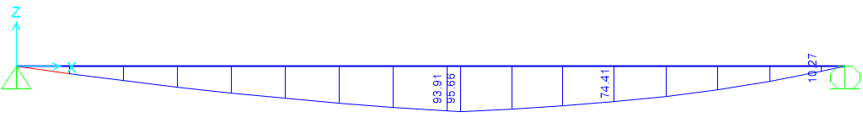
\includegraphics[width=0.9\linewidth]{images/viguetas/MOM-11C.png}
                \caption{Diagrama de momento (1.2D+1.6L) para la viga auxiliar V-11 de cubierta}
                \label{fig:Mom V-11 EP}
            \end{figure}
            
            \item \textbf{Viga auxiliar 12}\\
            \begin{figure}[H]
                \centering
                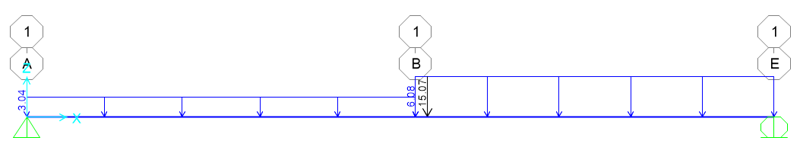
\includegraphics[width=0.9\linewidth]{images/viguetas/V-12C.png}
                \caption{Diagrama de carga (1.2D+1.6L) para la viga auxiliar V-12 de cubierta}
                \label{fig:W V-12 EP}
            \end{figure}
            
            \begin{figure}[H]
                \centering
                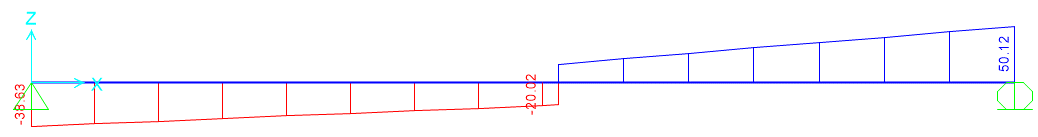
\includegraphics[width=0.9\linewidth]{images/viguetas/CORT-12C.png}
                \caption{Diagrama de cortante (1.2D+1.6L) para la viga auxiliar V-12 de cubierta}
                \label{fig:Cort V-12 EP}
            \end{figure}
            
            \begin{figure}[H]
                \centering
                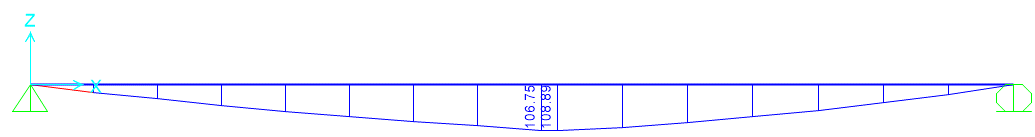
\includegraphics[width=0.9\linewidth]{images/viguetas/MOM-12C.png}
                \caption{Diagrama de momento (1.2D+1.6L) para la viga auxiliar V-12 de cubierta}
                \label{fig:Mom V-12 EP}
            \end{figure}
            
            
            \item \textbf{Viga auxiliar 13}\\
            \begin{figure}[H]
                \centering
                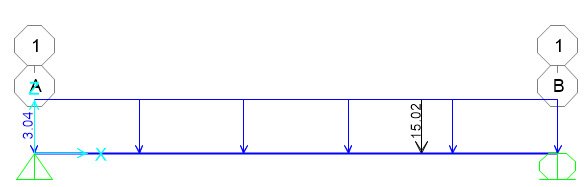
\includegraphics[width=0.9\linewidth]{images/viguetas/V-13C.png}
                \caption{Diagrama de carga (1.2D+1.6L) para la viga auxiliar V-13 de cubierta}
                \label{fig:W V-13 EP}
            \end{figure}
            
            \begin{figure}[H]
                \centering
                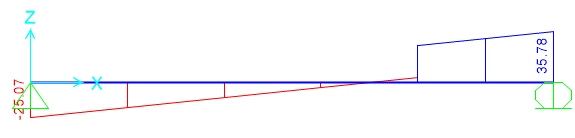
\includegraphics[width=0.9\linewidth]{images/viguetas/CORT-13C.png}
                \caption{Diagrama de cortante (1.2D+1.6L) para la viga auxiliar V-13 de cubierta}
                \label{fig:Cort V-13 EP}
            \end{figure}
            
            \begin{figure}[H]
                \centering
                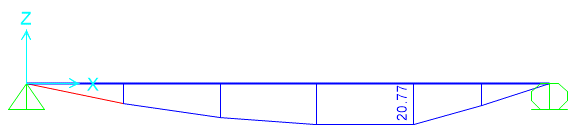
\includegraphics[width=0.9\linewidth]{images/viguetas/MOM-13C.png}
                \caption{Diagrama de momento (1.2D+1.6L) para la viga auxiliar V-13 de cubierta}
                \label{fig:Mom V-13 EP}
            \end{figure}
            
            \item \textbf{Viga auxiliar 14}\\
            \begin{figure}[H]
                \centering
                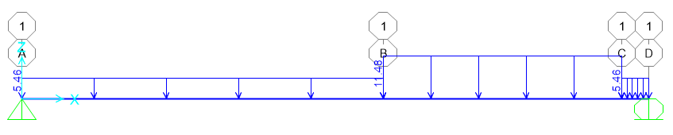
\includegraphics[width=0.9\linewidth]{images/viguetas/V-14C.png}
                \caption{Diagrama de carga (1.2D+1.6L) para la viga auxiliar V-14 de cubierta}
                \label{fig:W V-14 EP}
            \end{figure}
            
            \begin{figure}[H]
                \centering
                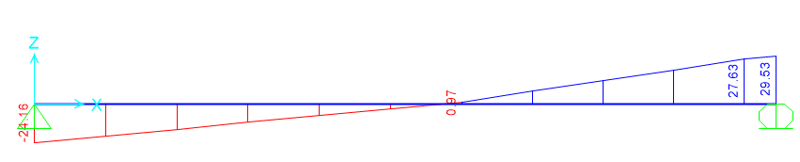
\includegraphics[width=0.9\linewidth]{images/viguetas/CORT-14C.png}
                \caption{Diagrama de cortante (1.2D+1.6L) para la viga auxiliar V-14 de cubierta}
                \label{fig:Cort V-14 EP}
            \end{figure}
            
            \begin{figure}[H]
                \centering
                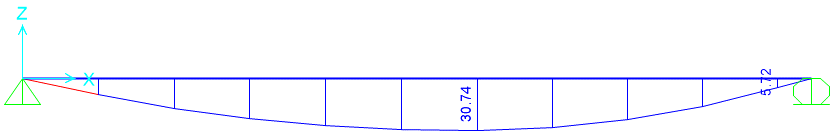
\includegraphics[width=0.9\linewidth]{images/viguetas/MOM-14C.png}
                \caption{Diagrama de momento (1.2D+1.6L) para la viga auxiliar V-14 de cubierta}
                \label{fig:Mom V-14 EP}
            \end{figure}
            
\end{itemize}